\section{Introduction}

\label{sec:intro}
\alida, which is the acronym for {\it Advanced Library for Integrated Development of Data Analysis Applications}, 
is the name of our integrated concept to ease the development and application of data analysis algorithms. 
For use in practice the concept is implemented in terms of a software library. 
This \alida library on the one hand allows for an automatic generation of
generic user interfaces for implemented algorithms, and on the other hand
subsumes the fully automatic documentation of data analysis processes performed
using functionality from the library.
The underlying core of the \alida concept is given by an interpretation of data
analysis processes as a sequence of data manipulations solely performed by
functional units, called {\em operators} in \alida. 
Given a generic framework for the implementation of operators in \alida, these
can be handled, i.e.~configured and executed, in a standardized manner.
This results in a wide range of useful features for programmers as well as users.

The operator concept, with the operators as the central places of data
manipulation and a unified invocation procedure, allows to monitor all data
manipulations taking place during a data analysis process. Additionally, all
objects ever manipulated are registered within the system and can be linked to
their manipulating operators.
An automatic documention of analysis procedures is supposed to subsume all
input and output objects involved in the execution of operators, all
manipulations performed with all their relevant parameters, the flow of data,
and also software versions as used. All this information is summarized in
the {\em processing graph}, which is implicitly defined by any data
analysis process. 
As manipulative actions can either work sequentially or in parallel on
data items, the processing graph is given by an acyclic directed graph.
Its nodes are associated with the different operations applied to the data, and
the edges in between represent the operators' ordering and the overall flow of
data and control. This representation is shown in Fig.~\ref{fig:DAG} for an
example graph.
As \alida allows to collect all relevant data for extracting processing
graphs due to its operator concept and the standardized invocation procedure for
operators, it allows to make the processing graph explicit without
additional efforts to the programmer or user.
In particular, for each output object of any analysis process the processing
graph can subsequently be made explicit in terms of an XML representation. 
This allows for convenient visualization, reconstruction and verification of 
results at a later point in time, and also for long-term archiving, e.g., 
in databases.

\begin{figure}[t]
\centerline{
%\includegraphics[clip, trim= 80 40 95 60, width=0.85\textwidth]
%                {analyzeData-withoutFile-edited}
{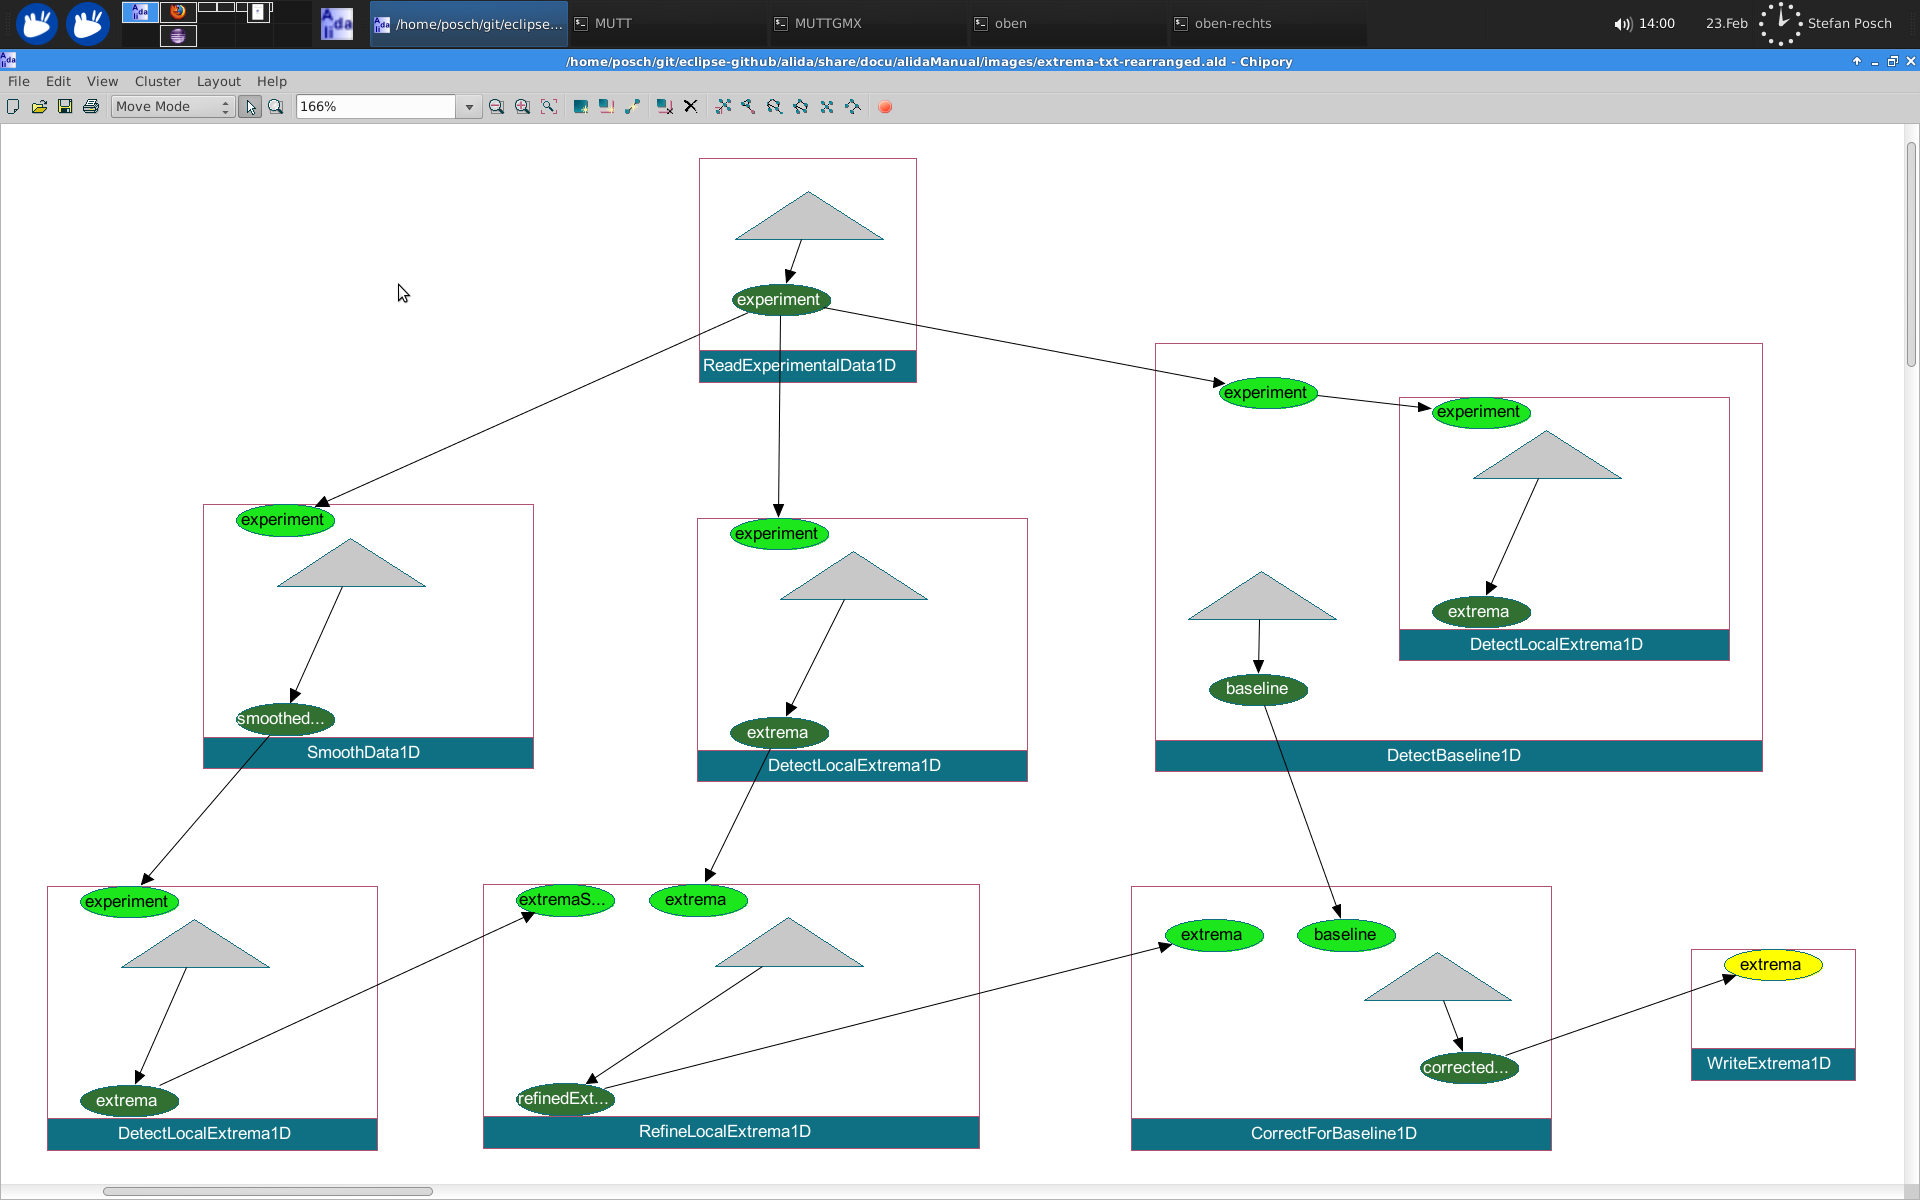
\includegraphics[clip, trim=200 140 200 110, width=0.85\textwidth]
                {extrema-txt-rearranged.png}}
}
\caption[Example of a processing graph.]{\label{fig:DAG}
Example processing graph representing the history
of operations for producing 
the data
object shown as yellow ellipse. Each operator invocation is respresented by a blue or, if the operator is temporarily
collapsed, to a violet rectangle. Light and dark green ellipses are input and
output ports of operators, gray triangles represent newly generated data objects. 
%A red triangle
%represents data read from disk which was accompanied by a processing graph of a
%former analysis procedure, which is connected to the current graph by a dashed
%edge. 
}
\end{figure}

While documenting analysis processes is helpful for verifying or reconstructing
results at later points in time, i.e., for long-term consistency and
preservation of data analysis outcomes, another important aspect of algorithm
development is the accessibility of algorithms and tools for programmers and users.
Usually neither developers of algorithms nor users are willing or able to spend much time on the 
implementation of user interfaces. \alida's operator concept and the
standardized configuration and execution procedures also offer a solution to
this problem by supporting the automatic generation of user interfaces for
operators.
More specifically, \alida's concept yields a suitable fundament for
automatically generating graphical and command line user interfaces which allow
to configure and execute all operators implemented in the \alida framework, as
well as to inspect the results of processing.
While a graphical interface mainly targets at immediate visual inspection of
operator configurations and results, a command line interface is useful, e.g.,
for parameter tuning or batch processing facilitated by scripts.

The framework for documentation and user interface generation is independent of
programming languages.
\alida currently features a mature implementation in Java.
%% and an early version in C++.
This implementation is shipped with a command line tool for running operators
from command line, and with a graphical user interface based on Java Swing,
which supports comfortable parameter editing and result data inspection in a
graphical framework, well-suited also for non-expert users.
In addition, the graphical editor \grappa is included which currently
supports the composition of flat workflows of operators and their partial or
complete execution (see Sec.~\ref{subsec:grappa}).
For convenience the configuration of operators, their execution and
the inspection of results are identical to the corresponding procedures
in the graphical user interface.
To inspect the automatically generated XML documentation, the graph
visualization tool \mtbc is available (see Appendix~\ref{app:chipory}).

In general, the \alida concept enforces minimal restrictions for users and
programmers, interferring as little as possible with usual software development
cycles, and resulting in an automatic documentation with a minimum of overhead.
\alida's concept is applicable to any data analysis process. 

%%Note that this manual is currently focused on the Java implementation of \alida,
%%but will include more details of the C++ implementation in the future.

Download of source code and binary bundels as well
as installation instructions are available on \alida's web-page, 
\url{http://www.informatik.uni-halle.de/alida}.
